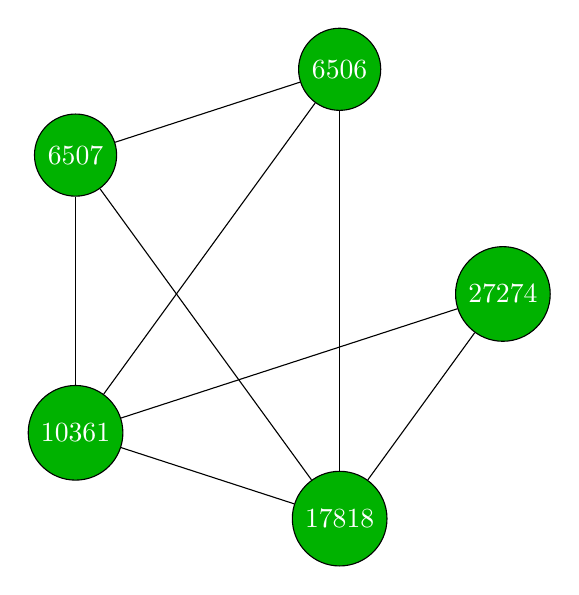
\begin{tikzpicture}
  \draw
    (0.000:3.000) node[fill=green!70!black, minimum size=4mm, circle, draw, text=white] (27274){27274}
    (72.000:3.000) node[fill=green!70!black, minimum size=2mm, circle, draw, text=white] (6506){6506}
    (144.000:3.000) node[fill=green!70!black, minimum size=2mm, circle, draw, text=white] (6507){6507}
    (216.000:3.000) node[fill=green!70!black, minimum size=2mm, circle, draw, text=white] (10361){10361}
    (288.000:3.000) node[fill=green!70!black, minimum size=2mm, circle, draw, text=white] (17818){17818};
  \begin{scope}[-]
    \draw (27274) to (10361);
    \draw (27274) to (17818);
    \draw (6506) to (6507);
    \draw (6506) to (10361);
    \draw (6506) to (17818);
    \draw (6507) to (10361);
    \draw (6507) to (17818);
    \draw (10361) to (17818);
  \end{scope}
\end{tikzpicture}
